\textbf{Problem:} Given $N$ rectangles in the plane, compute the measure (area) of their union.
\\
\\We solved the problem with the following algorithm which is visualized in figure~\ref{fig:segments}.

\subsection{Algorithm}

\begin{enumerate}
\item \label{enu:segments} Construct 4 segments for each rectangle consisting of a 'overlap' attribute initialized to 0 and has an associated list of rectangles that has a corner point at the segment. Initially the list only contains the rectangle the segment is constructed from. In total $4N$ segments are constructed. These segments are shown in the second picture in figure~\ref{fig:segments}. The 'overlap' attribute describes how large a part is overlapped by rectangles from the segment to the next segment (the one with the next $y$ value).
\item \label{enu:sorting} Sort segments by $x$ value, then by $y$. When sorting, all segments are points, therefore the $x$ value is well defined. The sorting can be done using two external mergesorts. A \emph{strip} is created for all different values of $x$. A strip contains a 'width' attribute and a list of segments. Initially a strip has a width of 0 and all the segments that has the given $x$ value.
\item \label{enum:combine} Combine $d$ strips until only one strip remains by (shown in the last three pictures in figure~\ref{fig:segments})
    \begin{enumerate}
        \item Iterating through all $d$ strips by $y$ value. Each iteration combines between 1 and $d$ segments. I.e. there might only be one segment with the next lowest $y$ value or there might be a segment in all $d$ strips with the next lowest $y$.
        \item Two arrays $E$ and $W$ are updated while iterating the strips. $E$ contains $d$ counts where $E_i>0$ means that some rectangle is covering the horizontal area strip $i$ covers. $W$ contains $d-1$ counts where $W_i>0$ means that some rectangle is covering the horizontal space between strip $i$ and strip $i+1$. These counts are easily updated when the rectangles in segments are iterated. If a rectangle in a segment has a start point at the segment and the rectangle overlaps strip $i$  then $E_i$ is incremented. If it is an endpoint then the count is decremented. Similarly for $W$.
        \item All the rectangles in the segments that are combined will be stored in the combined segment. The overlap of the combined segment is computed from the $E$, $W$ and the 'overlap' attributes of the combined segments.
    \end{enumerate}
\item \label{enu:calculate} Calculate the total area by summing the vertical difference between segments $s_{y}$ and $s_{y+1}$ multiplied by the 'overlap' attribute of $s_{y}$.
\end{enumerate}

We have verified the correctness of the algorithm by implementing it in-memory.

\subsection{Analysis}

Step \ref{enu:segments} reads all rectangles once and writes $4N$ segments to disk. This uses $O(\frac{N}{B})$ I/Os in total. The double sorting done in step \ref{enu:sorting} is done in the usual sorting bound. The combine step in \ref{enum:combine} is performed $O(\log_{d}{N})$ times because the algorithm starts with $O(N)$ strips. Each time, all segments and their associated rectangles are read once. Segments are combined which reduces the number of segments but the number of rectangles is kept constant ($4N$). Therefore, one combine step can be done in $O(\frac{N}{B})$ I/Os. In total for all the combine steps, the upper bound for I/Os is $O(\frac{N}{B}\log_{d}{N}$). The final step, step \ref{enu:calculate}, can be done with $O(\frac{N}{B})$ I/Os.

By using $d = \frac{M}{B}$ (possible because we can have $\frac{M}{B}$ buffered streams open), the total I/Os becomes $O(\frac{N}{B}\log_{\frac{M}{B}}{N})$. Observe that $\frac{N}{B}\log_{\frac{M}{B}}{N}=\frac{N}{B}(\log_{\frac{M}{B}}{\frac{N}{B}}+\log_{\frac{M}{B}}{B})$. The tall cache assumption implies that $N>B^2$, so in total we have $O(\frac{N}{B}\log_{\frac{M}{B}}{\frac{N}{B}})=O(sort(N))$ I/Os.

\begin{figure}[h!]
  \centering
  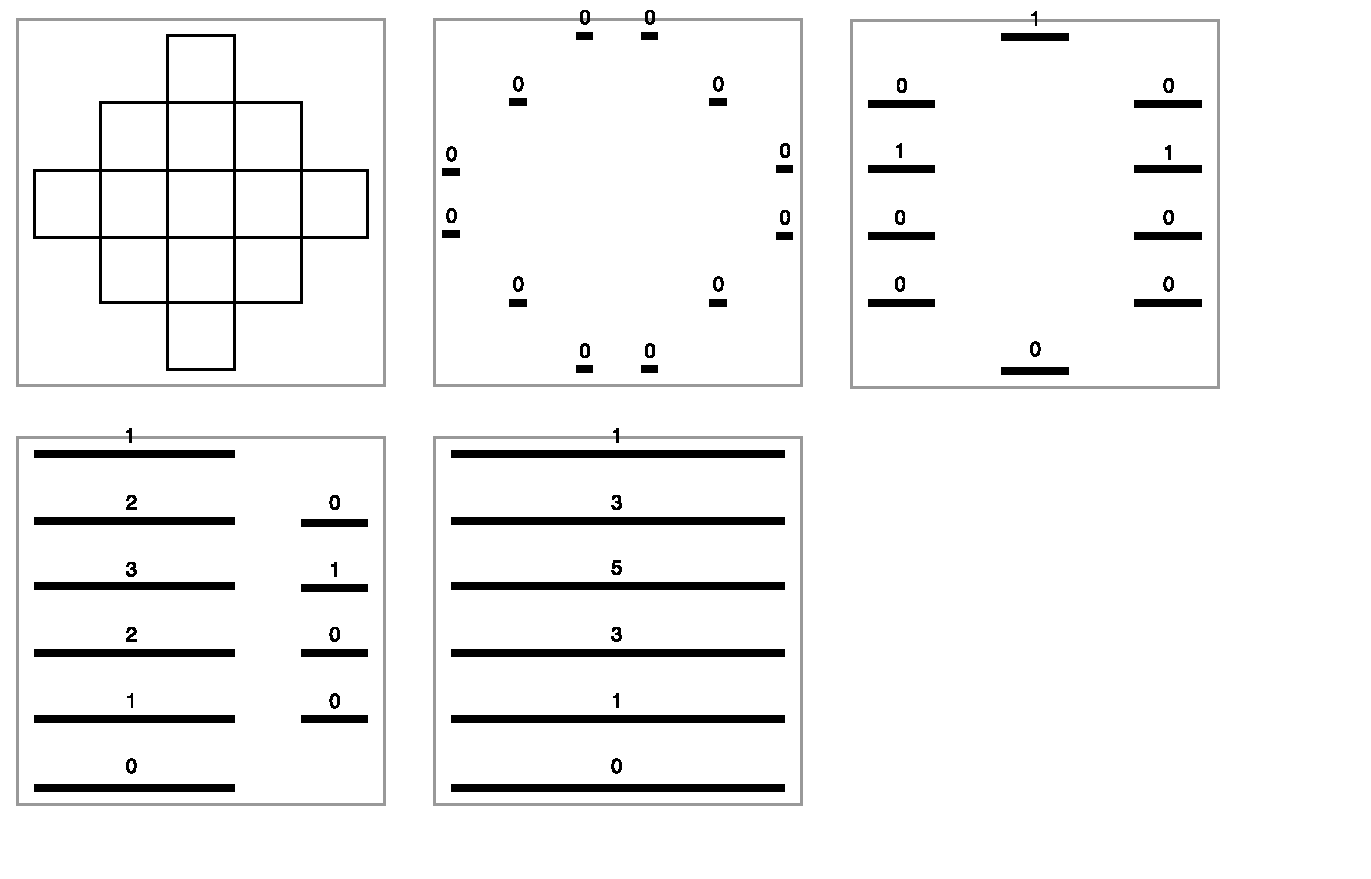
\includegraphics[width=1.12\textwidth]{images/Segments}
  \caption{An execution of the algorithm with $d = 2$.}
  \label{fig:segments}
\end{figure}